%%%%%%%%%%%%%%%%%%%%%%%%%%%%%%%%%%%%%%%%%
% Beamer Presentation
% LaTeX Template
% Version 1.0 (10/11/12)
%
% This template has been downloaded from:
% http://www.LaTeXTemplates.com
%
% License:
% CC BY-NC-SA 3.0 (http://creativecommons.org/licenses/by-nc-sa/3.0/)
%
%%%%%%%%%%%%%%%%%%%%%%%%%%%%%%%%%%%%%%%%%

%----------------------------------------------------------------------------------------
%	PACKAGES AND THEMES
%----------------------------------------------------------------------------------------

\documentclass{beamer}

\mode<presentation> {

% The Beamer class comes with a number of default slide themes
% which change the colors and layouts of slides. Below this is a list
% of all the themes, uncomment each in turn to see what they look like.

%\usetheme{default}
%\usetheme{AnnArbor}
%\usetheme{Antibes}
%\usetheme{Bergen}
%\usetheme{Berkeley}
%\usetheme{Berlin}
%\usetheme{Boadilla}
%\usetheme{CambridgeUS}
\usetheme{Copenhagen}
%\usetheme{Darmstadt}
%\usetheme{Dresden}
%\usetheme{Frankfurt}
%\usetheme{Goettingen}
%\usetheme{Hannover}
%\usetheme{Ilmenau}
%\usetheme{JuanLesPins}
%\usetheme{Luebeck}
%\usetheme{Madrid}
%\usetheme{Malmoe}
%\usetheme{Marburg}
%\usetheme{Montpellier}
%\usetheme{PaloAlto}
%\usetheme{Pittsburgh}
%\usetheme{Rochester}
%\usetheme{Singapore}
%\usetheme{Szeged}
%\usetheme{Warsaw}
\usepackage[flushleft]{threeparttable}
% As well as themes, the Beamer class has a number of color themes
% for any slide theme. Uncomment each of these in turn to see how it
% changes the colors of your current slide theme.

%\usecolortheme{albatross}
%\usecolortheme{beaver}
%\usecolortheme{beetle}
%\usecolortheme{crane}
%\usecolortheme{dolphin}
%\usecolortheme{dove}
%\usecolortheme{fly}
%\usecolortheme{lily}
%\usecolortheme{orchid}
%\usecolortheme{rose}
%\usecolortheme{seagull}
%\usecolortheme{seahorse}
%\usecolortheme{whale}
\usecolortheme{wolverine}

%\setbeamertemplate{footline} % To remove the footer line in all slides uncomment this line
%\setbeamertemplate{footline}[page number] % To replace the footer line in all slides with a simple slide count uncomment this line

%\setbeamertemplate{navigation symbols}{} % To remove the navigation symbols from the bottom of all slides uncomment this line
}

\usepackage{graphicx} % Allows including images
\usepackage{booktabs} % Allows the use of \toprule, \midrule and \bottomrule in tables
\usepackage{amsmath}

%----------------------------------------------------------------------------------------
%	TITLE PAGE
%----------------------------------------------------------------------------------------

\title[The Rise in Returns to Skill?]{The Rise in Returns to Skill? \\ \large{A Modern Regression Analysis of Wage Inequality in the Current Population Survey (CPS)}} % The short title appears at the bottom of every slide, the full title is only on the title page

\author{Senan Hogan-H.} % Your name
\institute[ECON 190: Senior Seminar in Economics] % Your institution as it will appear on the bottom of every slide, may be shorthand to save space
{
ECON 190, Pomona College\\ % Your institution for the title page
\medskip
\textit{senan.hoganhennessy@pomona.edu} % Your email address
}
\date{25 April 2018} % Date, can be changed to a custom date

\begin{document}

\begin{frame}
\titlepage % Print the title page as the first slide
\end{frame}

\begin{frame}
\frametitle{Overview} % Table of contents slide, comment this block out to remove it
\tableofcontents % Throughout your presentation, if you choose to use \section{} and \subsection{} commands, these will automatically be printed on this slide as an overview of your presentation
\end{frame}

%----------------------------------------------------------------------------------------
%	PRESENTATION SLIDES
%----------------------------------------------------------------------------------------

%------------------------------------------------
\section{Research Motivation} % Sections can be created in order to organize your presentation into discrete blocks, all sections and subsections are automatically printed in the table of contents as an overview of the talk
%------------------------------------------------

\subsection{Research Question} % A subsection can be created just before a set of slides with a common theme to further break down your presentation into chunks
%------------------------------------------------

\begin{frame}
\frametitle{Research Question}
\begin{itemize} \pause
\item Income inequality has been rising rapidly since the 1960s. \pause
\item What is driving this rise in inequality? \pause
\item How can standard statistical methods explain rising inequality?
\end{itemize}
\end{frame}

%------------------------------------------------

\begin{frame}
\frametitle{Research Question}
\begin{itemize} 
\item Income inequality has been rising rapidly since the 1960s.
\item What is driving this rise in inequality? 
\item How can non-standard statistical methods explain rising inequality?
\end{itemize}
\end{frame}

%------------------------------------------------
\subsection{Recent Trends}
\begin{frame}
\frametitle{Recent Trends}
\pause
\begin{figure}
  \centering
  \caption{Indexed Real Hourly Wage by Percentile, 1980-2016.}
  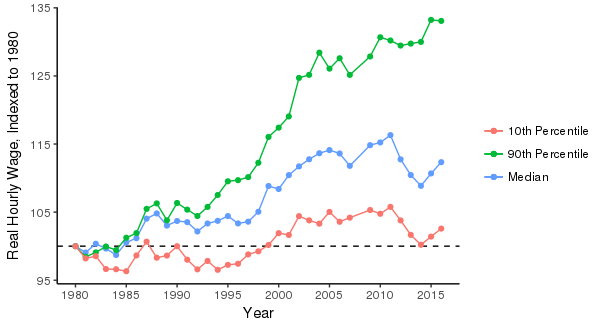
\includegraphics[width=9.5cm, height=5cm]{Ineq_graph.png}
\end{figure}
\end{frame}
%------------------------------------------------

\begin{frame}
\frametitle{Recent Trends}
\pause
\begin{figure}[H]
  \centering
  \caption{Ratio of Wage Between 90th and 10th Percentiles, 1980-2016.}
  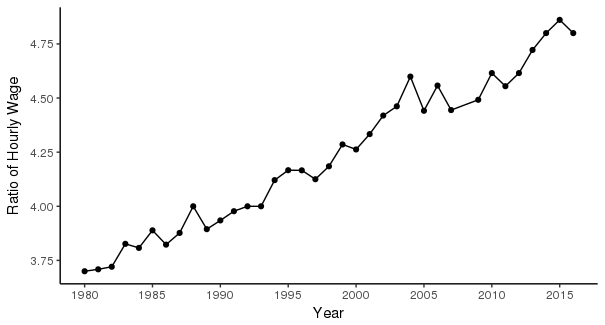
\includegraphics[width=9.5cm, height=5cm]{Ratio_plot1.png}
\end{figure} 
\end{frame}

%------------------------------------------------
\subsection{Literature review}
\begin{frame}
\frametitle{Previous Research}
\begin{itemize}
\pause
\item Juhn, Murphy, Pierce (1993, JMP 1993 henceforth) document rising wage inequality, and give a decomposition method attributing most of rising in inequality to rise in return to skill
\pause 
\item My research adjusts the JMP decomposition to modern regression methods
\end{itemize}
\end{frame}


%------------------------------------------------
\section{Methodology}

%Data Section, describe data set
%Specification and Specification simplified
%------------------------------------------------
\subsection{Data Section}
\begin{frame}
\frametitle{Data - March CPS}
\pause
\begin{figure}[H]
  \centering
  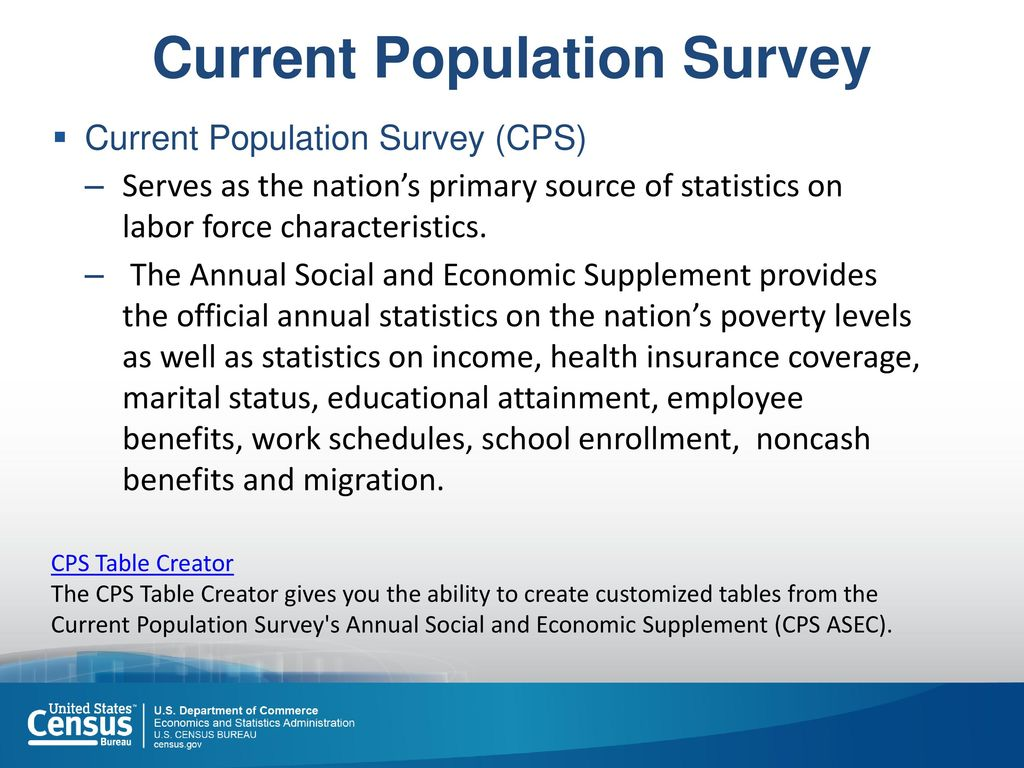
\includegraphics[width=9.5cm, height=6cm]{Current+Population+Survey.jpg}
\end{figure} 
\footnotesize{Used the CEPR March CPS extracts.  (accessed 2018)}
\end{frame}

%------------------------------------------------
\subsection{Decomposition Methods}
\begin{frame}
\frametitle{JMP Decomposition}
\pause
Standard linear model for predicting a measure of wages individual years:
\begin{equation}
Y_{it} = \mathbf{X}_{it}\beta_t + \varepsilon_{it}
\end{equation}
\pause
Consider returns to observed characteristics constant over the entire time period:
\begin{equation}
Y_{it} = \mathbf{X}_{it}\bar{\beta} + \varepsilon_{it}
\end{equation} \\
\pause
Note: \pause $\bar{\beta} \neq \beta_t$, for $t = 1980, \dots, 2016$
\end{frame}

%------------------------------------------------

\begin{frame}
\frametitle{JMP Decomposition}
\begin{center} \pause 
(observed income distribution) \\$Y_{it} = $  \vspace{0.5cm} \\  \pause 
(predicted income distribution, under fixed returns) \\ $\mathbf{X}_{it}\bar{\beta}$ \\
$+$ \pause \\
(difference to predicted income distribution, under variable returns) \\ $\mathbf{X}_{it}(\beta_t - \bar{\beta})$ \\
$+$ \pause \\
(residuals, unexplained factors) \\
$\varepsilon_{it}$
\end{center}


\end{frame}


%------------------------------------------------

\begin{frame}
\frametitle{JMP Decomposition}
So that the distribution of income is the sum of three components:
\begin{equation}
Y_{it} = \mathbf{X}_{it}\bar{\beta} + \mathbf{X}_{it}(\beta_t - \bar{\beta}) + \varepsilon_{it}
\end{equation} 
\pause
$\Rightarrow$ This approach relies heavily on the variables in $\mathbf{X}_{it}$ or even prediction method used.
\pause

$\Rightarrow$ Perhaps we could use more than OLS?
\end{frame}

%------------------------------------------------

\subsection{Prediction Methods}
\begin{frame}
\frametitle{Prediction Methods}
\pause
Mincer Wage equation, dating to Mincer (1954, 1972):
\begin{equation}
Y_{it}  = Y_0 + \rho_t s_{it} +\beta_{1t} x_{it} + \beta_{2t} x_{it}^2 + \varepsilon_{it}
\end{equation}
\pause 
Adjusted Mincer wage equation, proposed by Lemieux (2006):
\begin{equation}
Y_{it}  = Y_0 + \rho_{1t} s_{it} + \rho_{2t} s_{it}^2 + \beta_{1t} x_{it} + \beta_{2t} x_{it}^2 + \beta_{3t} x_{it}^3 + \beta_{4t} x_{it}^4 + \varepsilon_{it}
\end{equation}
\end{frame}

%------------------------------------------------
\begin{frame}
\frametitle{Prediction Methods}
Novel prediction methods, tree-based regression.
\pause
\begin{figure}
  \centering
  \caption{Decision tree for real log wages, 2010-2016.}
  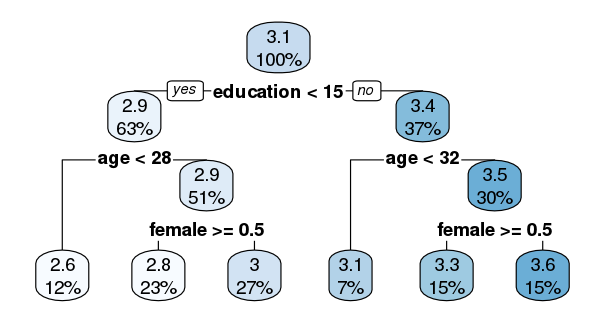
\includegraphics[width=8cm, height=4cm]{Rpat2010_2016.png}
\end{figure}
\pause
Random forest regression uses random sampling and builds a forest of decision trees to average across for predictions.
\end{frame}

%------------------------------------------------
\section{Results}
\subsection{Decomposition}
\begin{frame}
\frametitle{Results - Mincer Wage Equation}
\pause
\begin{figure}
  \centering
  \caption{Components of 90-10 Percentile Log Wage Differential.}
  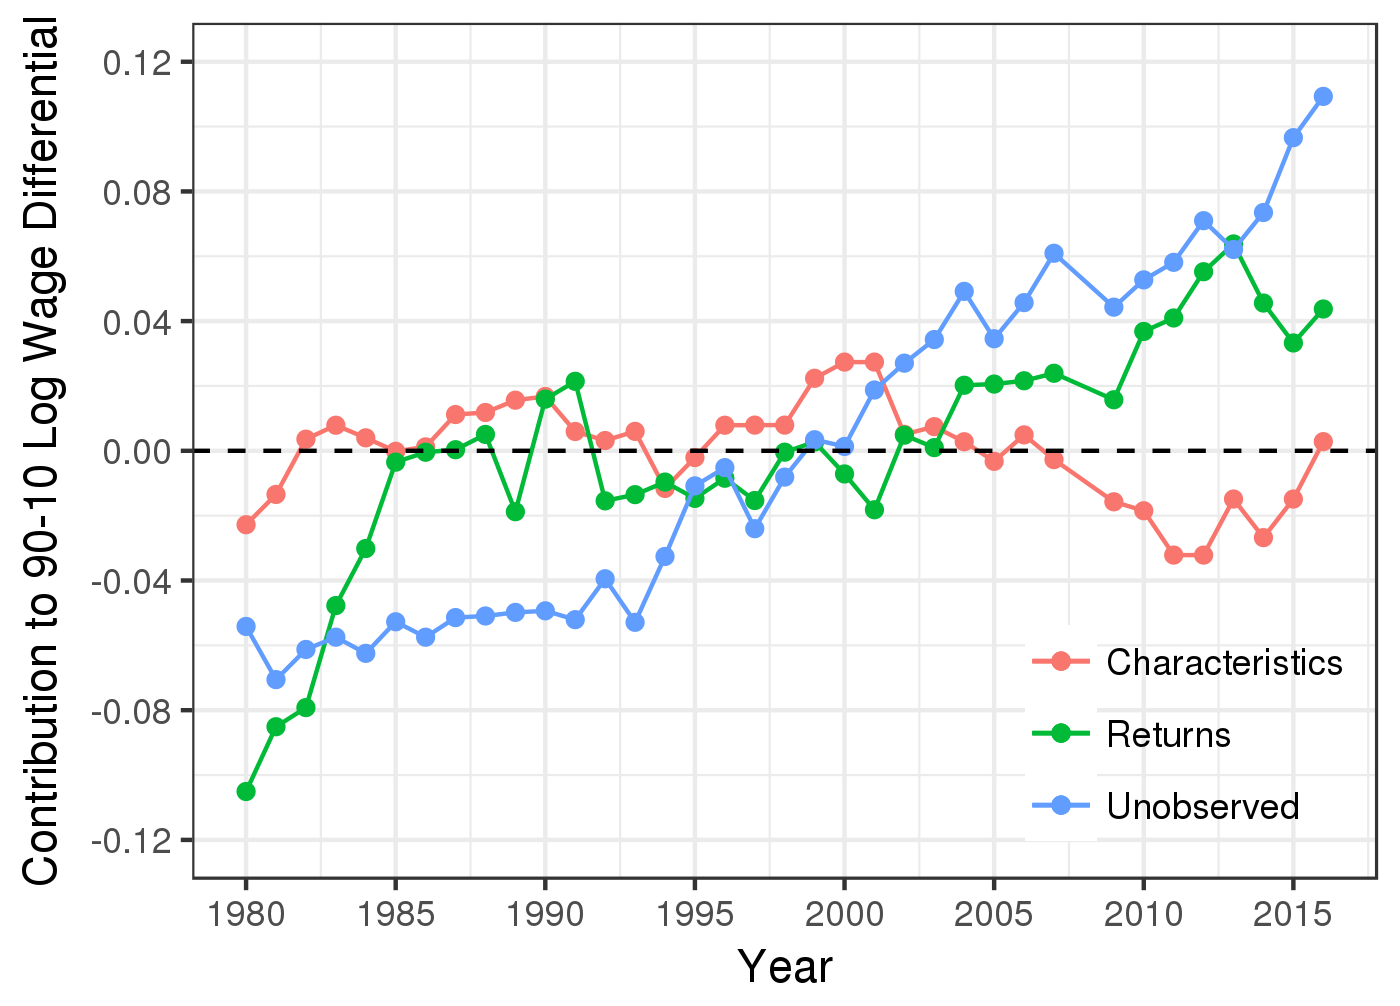
\includegraphics[width=8.8cm, height=5.5cm]{edit1.png}
\end{figure}
\end{frame}

%------------------------------------------------

\begin{frame}
\frametitle{Results - Adjusted Mincer Wage Equation}
\pause
\begin{figure}
  \centering
  \caption{Components of 90-10 Percentile Log Wage Differential.}
  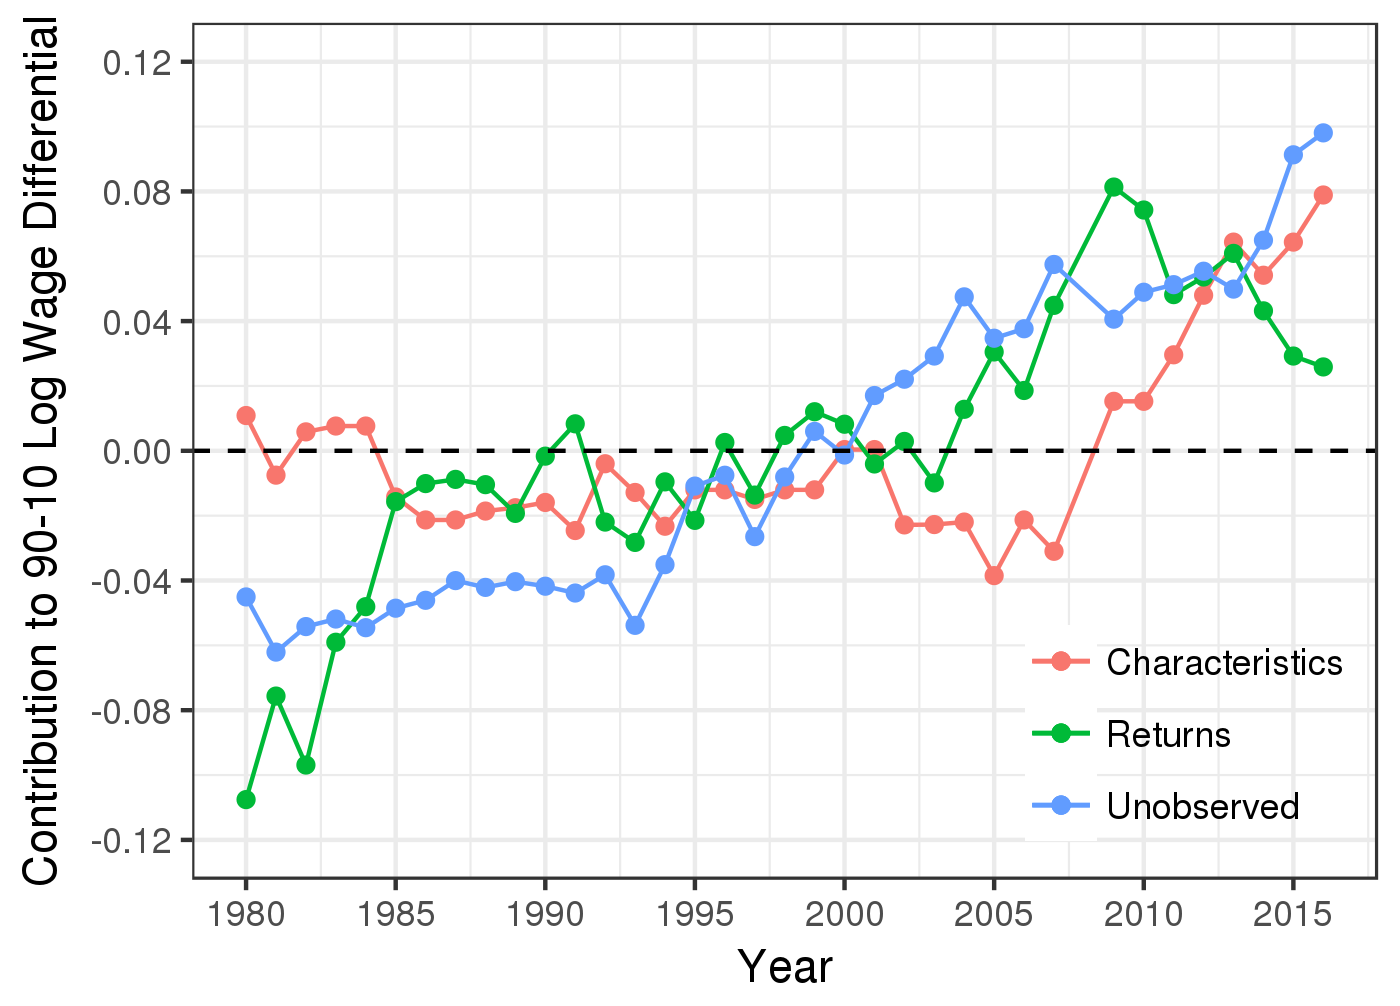
\includegraphics[width=8.8cm, height=5.5cm]{edit2.png}
\end{figure}
\end{frame}

%------------------------------------------------

\begin{frame}
\frametitle{Results - Random Forest Prediction}
\pause
\begin{figure}
  \centering
  \caption{Components of 90-10 Percentile Log Wage Differential.}
  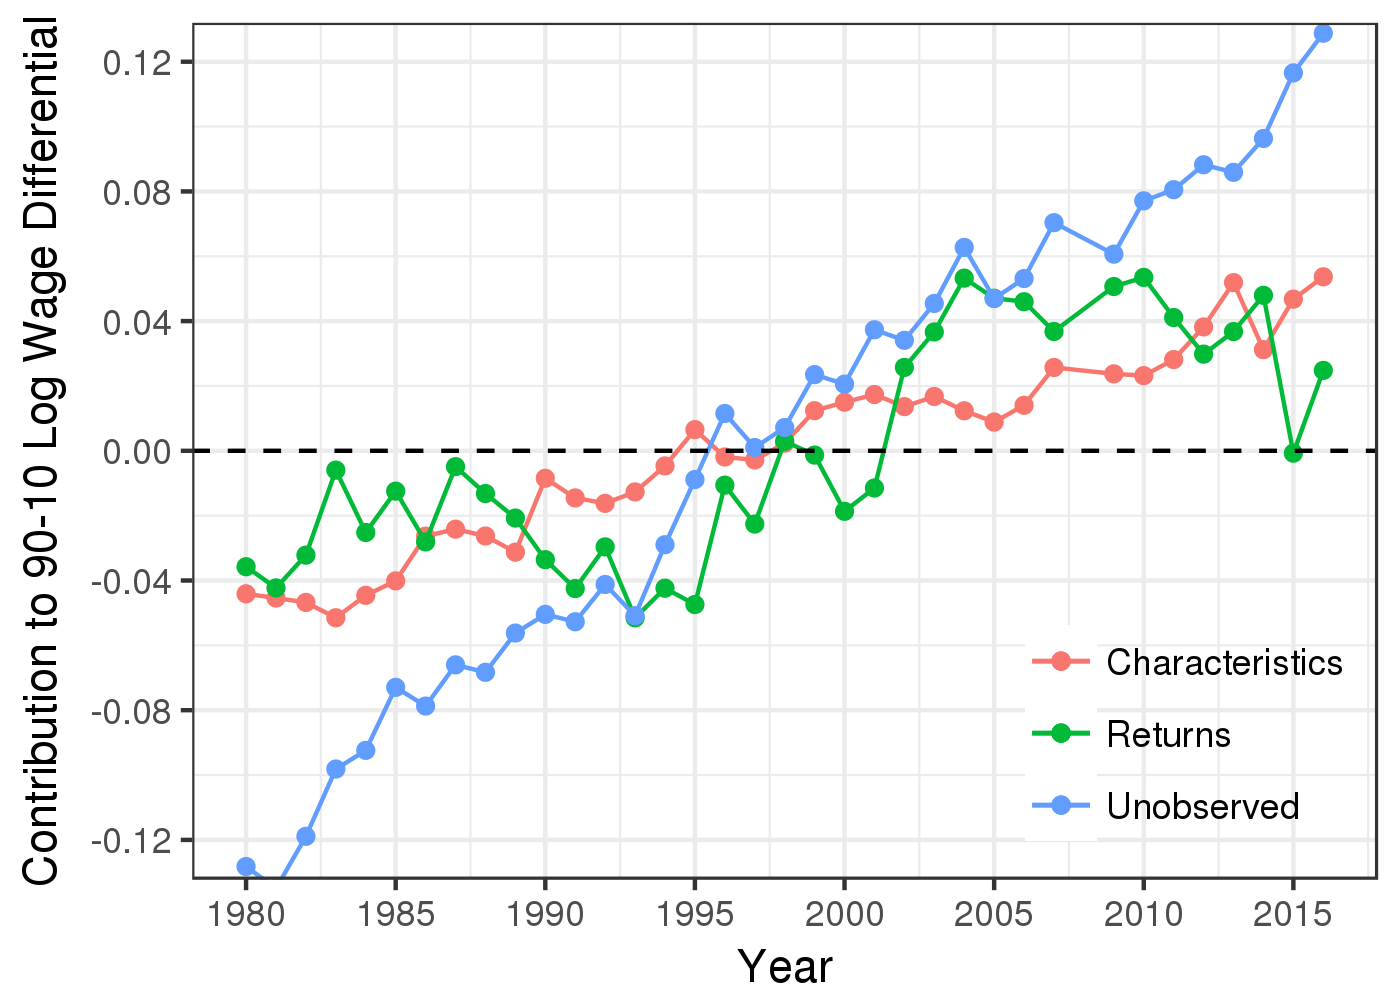
\includegraphics[width=8.8cm, height=5.5cm]{edit3.png}
\end{figure}
\end{frame}

%------------------------------------------------

\subsection{Variable Importance}
\begin{frame}
\frametitle{Results - Variable Importance}
\pause
\begin{figure}  
	\caption{Variable Importance in Random Forest Prediction, 1980--2016}
  \centering
  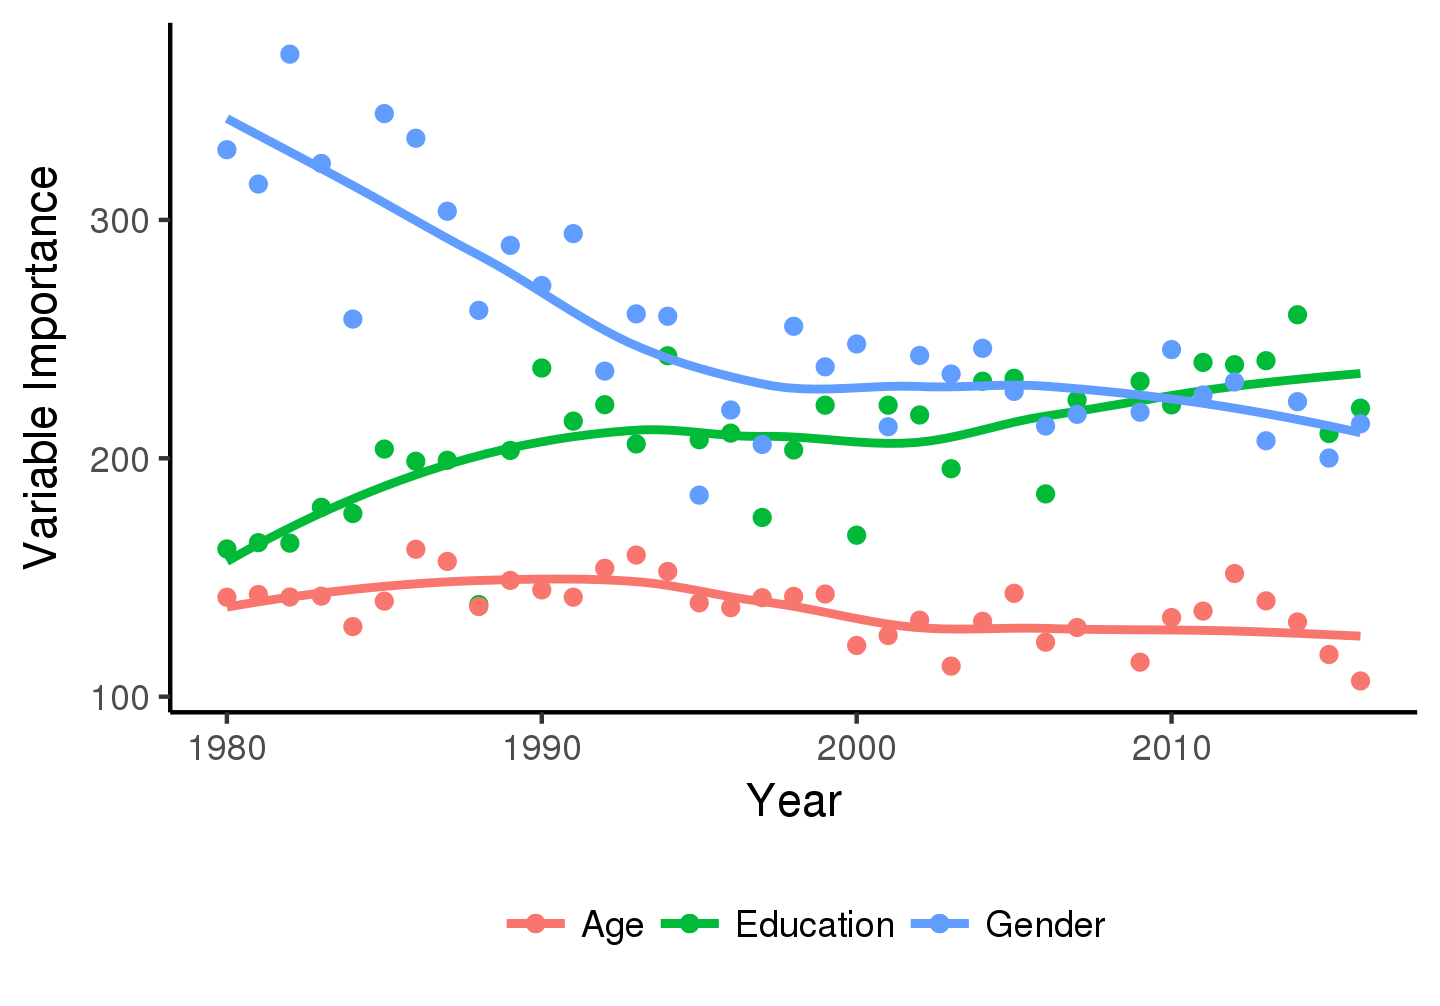
\includegraphics[width=0.7\textwidth]{importance_graph.png}
\end{figure}
\end{frame}

%------------------------------------------------
\section{Summary}
\subsection{Overview of Results}
\begin{frame}
\frametitle{Summary}
\begin{itemize}
\pause
\item Distribution of residuals and thus ``unobserved'' skill depends largely on prediction method used. \vspace{10mm} 
\pause
\item Role of unobserved factors play a larger role post-1980's and more so in better prediction methods. \vspace{10mm} 
\pause
\item Education is more and more important in random forest prediction of wages, while gender's role reduces. \vspace{10mm} 
\end{itemize}
\end{frame}

%------------------------------------------------
\subsection{Discussion and Limitations}
\begin{frame}

\frametitle{Discussion and Limitations}
\pause
\begin{center}
Statistical properties? \\ \vspace{5mm} \pause
$E[\hat{\bar{\beta}}] =$ ? $= E[\hat{\beta}_t]$ \\ \vspace{5mm} \pause

$ \hat{\bar{\beta}} \xrightarrow[n \rightarrow \infty]{p} $ ? $ \xleftarrow[n \rightarrow \infty]{p} \hat{\beta}_t$ \hspace{1mm} \pause \\ \vspace{5mm}

Why just random forests?
\end{center}
\end{frame}

\begin{frame}
\frametitle{}
Thank you for listening \\ \vspace{10mm} 
\pause
Any questions?
\end{frame}

\end{document}